\documentclass{article}
\usepackage{amsmath}
\usepackage{graphicx}
\begin{document}
\graphicspath{ {./Images/} }
% Main Title
\title{Assignment 2}
\author{Aditya Gupta}
\date{\today}
\maketitle


\subsection*{38. Proving \( \lim_{x \to 0} (2 - 5x) = 2 \)}

We want to prove:
\[
\lim_{x \to 0} (2 - 5x) = 2
\]


\begin{enumerate}
    \item Start with the expression:
    \[
    |(2 - 5x) - 2| = |-5x|
    \]
    
    \item Simplify:
    \[
    |-5x| = 5|x|
    \]
    
    \item To make \(5|x| < \epsilon\), divide both sides by 5:
    \[
    |x| < \frac{\epsilon}{5}
    \]
    
    \item Therefore, choose \(\delta = \frac{\epsilon}{5}\).
    
\end{enumerate}

\textbf{Proof:}
Thus, for all \(x\) such that \(0 < |x| < \delta\), we have:
\[
|x| < \frac{\epsilon}{5}
\]
\[
5|x| < \epsilon
\]
\[
|-5x| < \epsilon
\]
\[
|(2 - 5x) - 2| < \epsilon
\]


This completes the epsilon-delta proof, proving $
\lim_{x \to 0} (2 - 5x) = 2
$

\subsection*{52. Proving \( \lim_{x \to 3} \sqrt{x+1} = 2 \)}

We want to prove:
\[
\lim_{x \to 3} \sqrt{x + 1} = 2
\]

\textbf{Proof:}

We need to show that for every \( \epsilon > 0 \), there exists a \( \delta > 0 \) such that if \( 0 < |x - 3| < \delta \), then:
\[
|\sqrt{x + 1} - 2| < \epsilon
\]

\begin{enumerate}
    \item Start with:
    \[
    |\sqrt{x + 1} - 2|
    \]
    
    \item Multiply and divide by the conjugate:
    \[
    |\sqrt{x + 1} - 2| = \frac{|(x + 1) - 2^2|}{|\sqrt{x + 1} + 2|}
    \]
    Simplifying the numerator gives:
    \[
   \frac{|x - 3|}{|\sqrt{x + 1} + 2|}
    \]
    
    \item Since $\sqrt{x+1}$ is always positive, we can remove it from the denominator removing it only increases the fraction:
    \[
    \frac{|x - 3|}{2}
    \]
    
    \item Choosing, \( \delta = 2 \epsilon \).
    
    \item Therefore, whenever \( 0 < |x - 3| < \delta = 2 \epsilon \), we have:
    \[
    |\sqrt{x + 1} - 2| < \epsilon
    \]
\end{enumerate}

This completes the proof.

\subsection*{ 54. Proving \( \lim_{x \to 0} g(x) = 0 \)}

We want to prove:
\[
\lim_{x \to 0} g(x) = 0
\]
for the function defined as:
\[
g(x) = \begin{cases} 
x & \text{if } x \text{ is rational} \\ 
0 & \text{if } x \text{ is irrational} 
\end{cases}
\]

\textbf{Proof:}

We need to show that for every \( \epsilon > 0 \), there exists a \( \delta > 0 \) such that whenever \( 0 < |x| < \delta \), it follows that:
\[
|g(x)| < \epsilon.
\]

\textbf{Taking Cases}:

\textbf{Case 1:} \(x\) is rational.

If \(x\) is rational, then \(g(x) = x\). Thus, we have:
\[
|g(x)| = |x|.
\]

For this case, we want to ensure that:
\[
|x| < \epsilon.
\]
We can choose \(\delta = \epsilon\). Then whenever \(0 < |x| < \delta\), we have:
\[
|g(x)| = |x| < \epsilon.
\]

\textbf{Case 2:} \(x\) is irrational.

If \(x\) is irrational, then \(g(x) = 0\). Thus, we have:
\[
|g(x)| = |0| = 0.
\]
Since \(0 < |g(x)| < \epsilon\) holds true for all \(\epsilon > 0\), we can choose any \(\delta > 0\) because the inequality is satisfied regardless of \(x\). Thus, we have proven $g(x)$ approaches 0 as $x \to 0$

\subsection*{61e. Inductive proof of power rule}


\textbf{Step 1: Base Case ($n = 1$)} \\
For $n = 1$, the derivative is:
\[
\frac{d}{dx}(x) = \lim_{h \to 0} \frac{(x+h) - x}{h} = \lim_{h \to 0} \frac{h}{h} = 1
\]
\[
\frac{d}{dx}x = 1 \cdot x^{0} = 1
\]
Thus, the base case holds.

\textbf{Step 2: Inductive Hypothesis} \\
Assume that for some $n = k$, the power rule holds:
\[
\frac{d}{dx}(x^k) = kx^{k-1}
\]

\textbf{Step 3: Inductive Step} \\
We now prove that the rule holds for $n = k+1$. Using the definition of the derivative, we have:
\[
\frac{d}{dx}(x^{k+1}) = \lim_{h \to 0} \frac{(x+h)^{k+1} - x^{k+1}}{h}
\]
We begin by factoring $(x+h)^{k+1} - x^{k+1}$ as:
\[
(x+h)^{k+1} - x^{k+1} = (x+h)(x+h)^k - x \cdot x^k
\]
Expanding:
\[
= x(x+h)^k + h(x+h)^k - x \cdot x^k
\]
Factoring and grouping terms involving $x$, we get:
\[
= x\left((x+h)^k - x^k\right) + h(x+h)^k
\]
Now, substitute this back into the limit:
\[
\frac{d}{dx}(x^{k+1}) = \lim_{h \to 0} \frac{x\left((x+h)^k - x^k\right) + h(x+h)^k}{h}
\]
We split the limit into two parts:
\[
= \lim_{h \to 0} \left( x \cdot \frac{(x+h)^k - x^k}{h} \right) + \lim_{h \to 0} \frac{h(x+h)^k}{h}
\]
The second term simplifies to:
\[
\lim_{h \to 0} (x+h)^k = x^k
\]
For the first term, by the inductive hypothesis:
\[
\lim_{h \to 0} \frac{(x+h)^k - x^k}{h} = kx^{k-1}
\]
Thus, the derivative becomes:
\[
\frac{d}{dx}(x^{k+1}) = x \cdot kx^{k-1} + x^k = kx^k + x^k = (k+1)x^k
\]
\newpage
\noindent\textbf{Conclusion:} \\
By induction, the power rule $\frac{d}{dx}(x^n) = nx^{n-1}$ holds for all positive integers $n$.

\subsection*{36. For what values of \( A \) is \( f \) continuous at \( x = 2 \)?}

Let \( f(x) = 
\begin{cases} 
A^2 x^2 & \text{if } x \leq 2 \\ 
(1-A)x & \text{if } x > 2 
\end{cases} \). 


If $f(x)$ is continuous,
\[
\lim_{x \to 2^-} f(x) = f(2) = \lim_{x \to 2^+} f(x).
\]

Calculating these limits, we find:

\[ f(2) = A^2(2^2) = 4A^2 \]
\[ \lim_{x \to 2^-} f(x) = 4A^2 \]
\[ \lim_{x \to 2^+} f(x) = 2(1-A) \]

Setting the limits equal gives the equation:

\[
4A^2 = 2(1-A).
\]

Solving the quadratic for \( A \), we obtain the values:

\[
A = 0.5, -1
\]


\subsection*{53}

To prove that if there is a constant \( B \) such that 

\[
|f(x) - f(c)| \leq B |x - c| :  x \in (c - p, c + p) 
\]

\noindent then \( f \) is continuous at \( x = c \).
\bigbreak
\noindent For every \( \epsilon > 0 \), there exists a \( \delta > 0 \) such that whenever \( |x - c| < \delta \), it follows that \( |f(x) - f(c)| < \epsilon \).
\begin{enumerate}


    \item Given: 

    \[
    |f(x) - f(c)| < \epsilon.
    \]

    \item We need to make

    \[
    B |x - c| < \epsilon.
    \]

    \[
    |x - c| < \frac{\epsilon}{B}.
    \]

    \item Thus we have to choose 

    \[
    \delta = \frac{\epsilon}{B}.
    \]

    \item Thus: 
    
    If \( |x - c| < \delta \), then:

    \[
    |x - c| < \frac{\epsilon}{B} \implies B |x - c| < \epsilon \implies |f(x) - f(c)| < \epsilon.
    \]

  Therefore, \( f \) is continuous at \( x = c \).
\end{enumerate}


\subsection*{36. Solving the limit:}$\lim_{x \to 0} \frac{\sin(ax)}{\sin(bx)} $.

Solution:

We begin by rewriting the expression as:

\[
\lim_{x \to 0} \frac{\sin(ax)}{\sin(bx)} = \lim_{x \to 0} \left( \frac{\sin(ax)}{ax} \cdot \frac{bx}{\sin(bx)} \cdot \frac{a}{b} \right).
\]

According to the Limit Statement 2.5.6:

\[
\lim_{x \to 0} \frac{\sin(kx)}{kx} = 1 \quad \text{for any constant } k.
\]

Thus, we have:

\[
\lim_{x \to 0} \frac{\sin(ax)}{ax} = 1 \quad \text{and} \quad \lim_{x \to 0} \frac{bx}{\sin(bx)} = 1.
\]

Substituting these into the limit expression, we get:

\[
\lim_{x \to 0} \frac{\sin(ax)}{\sin(bx)} = 1 \cdot 1 \cdot\lim_{x \to 0} \left(\frac{a}{b} \right) = \frac{a}{b}.
\]

Thus, the limit is:

\[
\lim_{x \to 0} \frac{\sin(ax)}{\sin(bx)} = \frac{a}{b}.
\]

\subsection*{43. Show that $\lim_{x \to 0} x sin(\frac{1}{x})$}

\[
0 \leq \left|xsin\left(\frac{1}{x}\right)\right| \leq |x|
\]

\[
\lim_{x\to0} 0 =  0
\]
\[
\lim_{x\to 0} |x| = 0
\]

Thus by the squeeze theorem, the $\lim_{x\to 0} \left|xsin\left(\frac{1}{x}\right)\right| = 0$
Since $\left|xsin\left(\frac{1}{x}\right)\right|$ approaches 0 as x $\to$ 0, so does $xsin\left(\frac{1}{x}\right)$
\[
\lim_{x \to 0}xsin\left(\frac{1}{x}\right) = 0
\]

\subsection*{46.}


\[
f(x) = 
\begin{cases} 
1 & \text{if } x \text{ is rational}, \\
0 & \text{if } x \text{ is irrational}.
\end{cases}
\]

We want to prove that:

\[
\lim_{x \to 0} x f(x) = 0.
\]

\begin{itemize}
    \item Step 1: We know that for all $x \in \mathbb{R}$, the function $x f(x)$ satisfies the following bounds:
    \[
    0 \leq x f(x) \leq |x|
    \]
    \item Step 2: Taking the limit as $x \to 0$ for each part of the inequality:
    \[
    \lim_{x \to 0} 0 = 0 \quad \text{and} \quad \lim_{x \to 0} |x| = 0
    \]
    \item Step 3: By the squeeze theorem, since $0 \leq x f(x) \leq |x|$ and both the lower and upper bounds tend to 0, we conclude:
    \[
    \lim_{x \to 0} x f(x) = 0
    \]
\end{itemize}


\[
\lim_{x \to 0} x f(x) = 0.
\]


\subsection*{Worksheet 5}

The following proof will be applied to the earth later.

\textbf{Proof}

\begin{enumerate}

\item Let \( C \) be a circle with center \( O \) and radius \( r \). Let \( P \) and \( Q \) be two points on the circumference such that \( Q \) is diametrically opposite \( P \). Let R be any point on the circle such that it makes an angle of x with the centre and P.


\item  Let \( T(x) \) be the temperature at point \( R \) and let \( T(0) \) be the temperature at point \( P \) and \( T(\pi) \) be the temperature at point \( Q \).

\item Let $f(x)$ be the temperature difference between any two diametrically opposite points.

\item As \( R \) moves around the circle, the angle \( x \) changes from \( 0 \) to \( \pi \). Thus, the domain of $f(x)$ is between 0 and $\pi$
   \[
   f(0) = P - Q
   \]
   \[
   f(\pi) = Q - R
   \]

Therefore, $f(0) = - f(\pi)$.

\item Let $f(0) = a$. Then $f(\pi) = -a$. Since $-a< 0 <a$, there will be some value $c$ such that $0<c<\pi$ and $f(c) = 0$ in the interval $[0,\pi]$

\item In the case that $f(0) = f(\pi)$, the proposition will be proved as $f(0)$ has to equal 0.

\item To apply this to the Earth. Follow this process(This assumes Earth to be a perfect sphere). Designate any great circle on the sphere as C. A great circle is the largest possible circle that can be inscribed in a sphere. And then one may simply follow the steps 1 to 6 

\end{enumerate}

\subsection*{Worksheet 6}
\begin{figure}[h!]
    \centering
    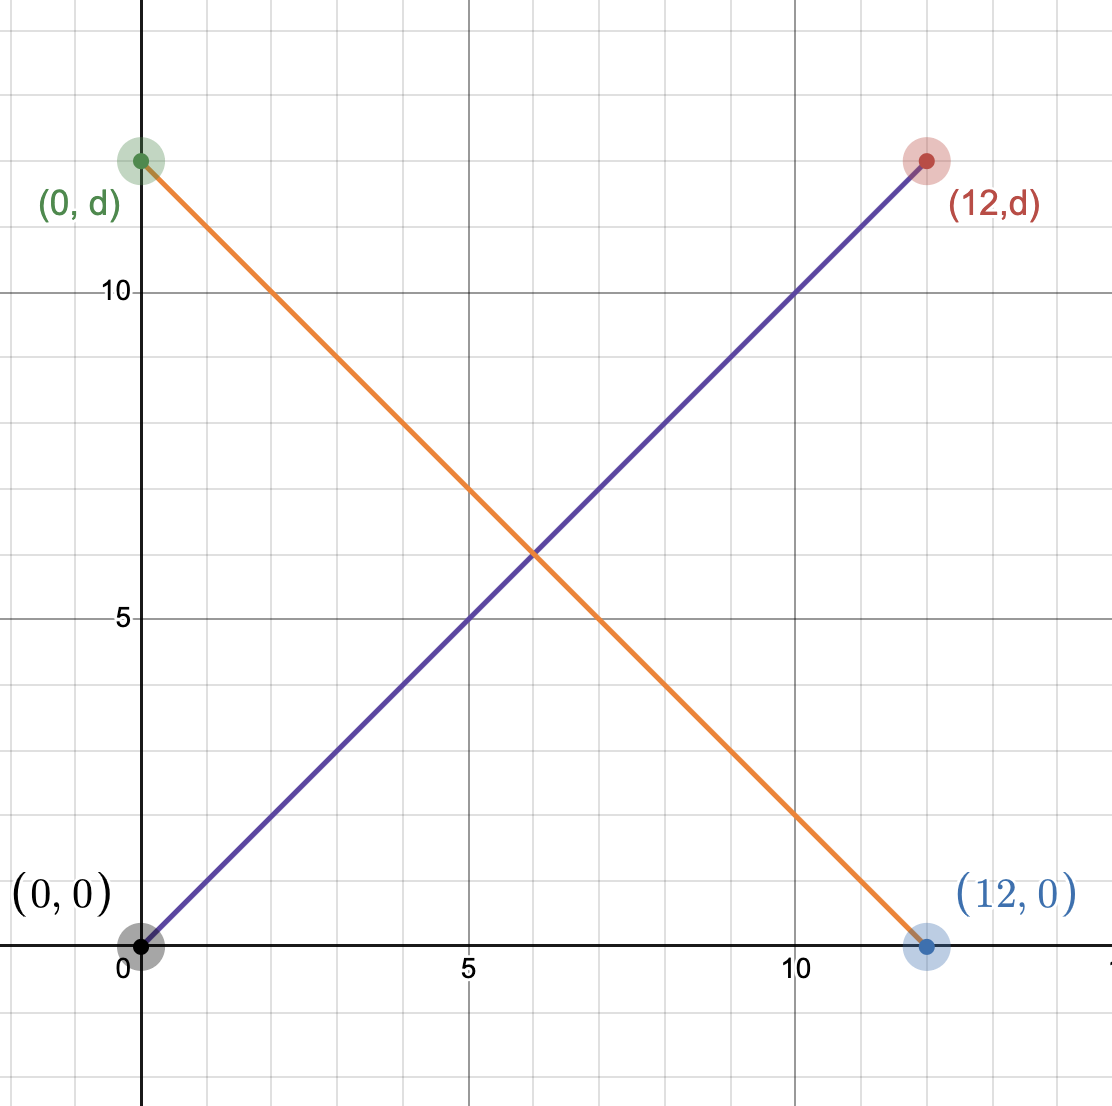
\includegraphics[width=0.5\linewidth]{PT.png}
\end{figure}
Referring to the position time graph:
\begin{itemize}
    \item The x-axis represents time from 0 to 12 hours
    \item The y-axis represents the position from 0 to d, d being the camp.
\end{itemize}

Two lines are drawn on the graph:
\begin{itemize}
    \item The purple line represents the hiker's position on the journey to the camp.
    \item The orange line represents the hiker's position on the journey back from the camp.
\end{itemize}

\noindent\textbf{Reasoning:}

Because both lines are continuous and one starts below the other at \( t = 0 \) and they swap positions at \( t = 12 \), the two curves must intersect at least once in the interval \( (0, 12) \). This crossing point corresponds to a time \( t \) where the hiker was at the same position on the trail on both the outbound and return journeys. The proof for the above reasoning is explored below 

\noindent\textbf{Proof:}

Let $f(x)$ be the function of the position as the hiker returns from the camp and let $g(x)$ be the function of the position as he makes the journey to the camp. Let $h(x) = f(x) - g(x)$. Thus, if we can find an example of $h(x) = 0$, we know that the hiker reached the same position at the same time on both days.

Firstly, we will find the domain and range of $h(x)$. 

\[
D: [0, 12]
\]
\[
R: [-d,d]
\]
According to the intermediate value theorem,
Since $-d < 0 < d$, there is a value $c$ such that $0 < c < 12$ and $f(c) = 0$

\end{document}
